\documentclass[10pt]{article}
\usepackage[T1]{fontenc}
\usepackage[utf8]{inputenc}
\usepackage{geometry}
\geometry{verbose,portrait,paperwidth=210mm,paperheight=297mm,tmargin=10mm,bmargin=15mm,lmargin=10mm,rmargin=10mm,headheight=0mm,headsep=0mm,footskip=5mm}
\usepackage[english]{babel}
\usepackage{amsmath}
\usepackage{amssymb}
\usepackage{graphicx}
\usepackage{color}
\usepackage{fancyhdr}
\usepackage{verbments}
\usepackage{fontspec}

\usepackage{tocloft}
\renewcommand{\cftsecleader}{\cftdotfill{\cftdotsep}}

\usepackage{hyperref}
\hypersetup{colorlinks=true, linktoc=all, linkcolor=blue}

\usepackage[toc]{multitoc}
\renewcommand*{\multicolumntoc}{2}
\setlength{\columnseprule}{0.4pt}
\setlength{\columnsep}{36pt}

\usepackage{multicol}
\usepackage{verbatim}

\usepackage{longtable}

\setlength\parindent{0mm}
\pagestyle{fancy}

%\definecolor{fcol}{RGB}{128, 128, 128}
\definecolor{fcol}{RGB}{ 64,   0, 128}
\definecolor{pcol}{RGB}{ 17, 128,  48}
\definecolor{gray}{RGB}{128, 128, 128}
\newcommand{\func}[1]{\textcolor{fcol}{\textbf{\fontspec{Anonymous Pro}#1}}}
\newcommand{\parm}[1]{\textcolor{pcol}{\fontspec{Anonymous Pro}#1}}

\begin{document}
\lhead{} \chead{} \rhead{}
\lfoot{} \cfoot{} \rfoot{\thepage}
\renewcommand{\headrulewidth}{0pt}
\renewcommand{\footrulewidth}{0pt}

\setmainfont{Candara}

\tableofcontents

\newpage

\section{qm3.maths}
\normalsize
\subsection[matrix]{matrix.py}
This module provides basic functionality to work with matrices. The whole module has been writen in python for
portabilty, but it will try to load different binary versions to improve effiency (see \func{matrix.version}).
Matrices are represented by a single list containing \textbf{all} the elements (even for symmetric ones) \textbf{by rows}. In those
functions where the matrix is expected to be square, only the amount of rows (\parm{row}) is needed as a
parameter. On the other wise, both number of rows and columns (\parm{col}) must be provided. Finally, the \func{inverse}
function returns the pseudo-inverse for non-square matrices.

\begin{pyglist}[language=python,fvset={frame=single}]
def norm( vec )

def dot_product( va, vb )

def cross_product( *vec )

def from_diagonal( lst, row )

def from_upper_diagonal_rows( lst, row )

# Import from fortran column-packed symmetric matrix upper diagonal
def from_upper_diagonal_columns( lst, row )

def get_row( mat, row, col, i )

def get_column( mat, row, col, j )

def add_row( mat, row, col, lst ):

def add_column( mat, row, col, lst ):

def mprint( mat, row, col, fmt = "%8.3lf" )

def det( mat, row )

def T( mat, row, col )

def mult( a_mat, a_row, a_col, b_mat, b_row, b_col )

def diag( mat, row )

def inverse( mat, row, col )
\end{pyglist}
The \func{diag} function is only available if a binary version of the module is active.

\footnotesize
\begin{pyglist}[language=python,fvset={frame=single}]
>>> import qm3.maths.matrix as matrix

>>> matrix.version
version macOS Accelerate

>>> matrix.norm( [ 1, 2, 3, 4 ] )
[0.18257418583505536, 0.3651483716701107, 0.5477225575051661, 0.7302967433402214]

>>> matrix.dot_product( [1., .0, .0], [.0, 1., .0] )
0.0

>>> matrix.cross_product( [1., .0, .0], [.0, 1., .0] ) )
[0.0, -0.0, 1.0]

>>> matrix.mprint( matrix.from_diagonal( [ 1 for i in range( 10 ) ], 10 ), 10, 10, "%3.1lf" )
10 rows x 10 columns
1.0 0.0 0.0 0.0 0.0 0.0 0.0 0.0 0.0 0.0 
0.0 1.0 0.0 0.0 0.0 0.0 0.0 0.0 0.0 0.0 
0.0 0.0 1.0 0.0 0.0 0.0 0.0 0.0 0.0 0.0 
0.0 0.0 0.0 1.0 0.0 0.0 0.0 0.0 0.0 0.0 
0.0 0.0 0.0 0.0 1.0 0.0 0.0 0.0 0.0 0.0 
0.0 0.0 0.0 0.0 0.0 1.0 0.0 0.0 0.0 0.0 
0.0 0.0 0.0 0.0 0.0 0.0 1.0 0.0 0.0 0.0 
0.0 0.0 0.0 0.0 0.0 0.0 0.0 1.0 0.0 0.0 
0.0 0.0 0.0 0.0 0.0 0.0 0.0 0.0 1.0 0.0 
0.0 0.0 0.0 0.0 0.0 0.0 0.0 0.0 0.0 1.0 

>>> matrix.mprint( matrix.from_upper_diagonal_rows( [5, 50, 25, 590, 262, 141], 3 ), 3, 3 )
3 rows x 3 columns
   5.000   50.000   25.000 
  50.000  590.000  262.000 
  25.000  262.000  141.000 

>>> matrix.mprint( matrix.from_upper_diagonal_columns( [5, 50, 590, 25, 262, 141], 3 ), 3, 3 )
3 rows x 3 columns
   5.000   50.000   25.000 
  50.000  590.000  262.000 
  25.000  262.000  141.000 

>>> m = [ 1, 2, 3, 4, 5, 6, 7, 8, 9 ]
>>> matrix.mprint( m, 3, 3 )
3 rows x 3 columns
   1.000    2.000    3.000 
   4.000    5.000    6.000 
   7.000    8.000    9.000 

>>> matrix.get_row( m, 3, 3, 1 )
[4, 5, 6]

>>> matrix.get_column( m, 3, 3, 1 )
[2, 5, 8]

>>> matrix.det( m, 3 )
0.0

>>> matrix.mprint( matrix.T( m, 3, 3 ), 3, 3 )
3 rows x 3 columns
   1.000    4.000    7.000 
   2.000    5.000    8.000 
   3.000    6.000    9.000 

>>> matrix.add_row( m, 3, 3, [ 10, 11, 12 ] )
>>> matrix.mprint( m, 4, 3 )
4 rows x 3 columns
   1.000    2.000    3.000 
   4.000    5.000    6.000 
   7.000    8.000    9.000 
  10.000   11.000   12.000 

>>> matrix.add_column( m, 4, 3, [ 13, 14, 15, 16 ] )
>>> matrix.mprint( m, 4, 4 )
4 rows x 4 columns
   1.000    2.000    3.000   13.000 
   4.000    5.000    6.000   14.000 
   7.000    8.000    9.000   15.000 
  10.000   11.000   12.000   16.000 

>>> matrix.mprint( matrix.mult( m, 4, 4, m, 4, 4 ), 4, 4 )
4 rows x 4 columns
 160.000  179.000  198.000  294.000 
 206.000  235.000  264.000  436.000 
 252.000  291.000  330.000  578.000 
 298.000  347.000  396.000  720.000 

>>> m = [ 1,2,7, 2,5,8, 7,8,15 ]
>>> matrix.mprint( m, 3, 3 )
3 rows x 3 columns
   1.000    2.000    7.000 
   2.000    5.000    8.000 
   7.000    8.000   15.000 

>>> val, vec = matrix.diag( m, 3 )
>>> val
[-2.2703605163750216, 1.4104400696875399, 21.859920446687475]

>>> matrix.mprint( vec, 3, 3 )
3 rows x 3 columns
   0.833    0.450    0.324 
   0.290   -0.852    0.437 
  -0.472    0.270    0.839 

>>> matrix.mprint( vec, 3, 3 )
3 rows x 3 columns
   0.833   -0.450    0.324 
   0.290    0.852    0.437 
  -0.472   -0.270    0.839 

>>> matrix.mprint( matrix.mult( vec, 3, 3, matrix.T( vec, 3, 3 ), 3, 3 ), 3, 3 )
3 rows x 3 columns
   1.000    0.000   -0.000 
   0.000    1.000   -0.000 
  -0.000   -0.000    1.000 

>>> matrix.mprint( matrix.mult( vec, 3, 3, matrix.mult(
    matrix.from_diagonal( val, 3 ), 3, 3, matrix.T( vec, 3, 3 ), 3, 3 ), 3, 3 ), 3, 3 )
3 rows x 3 columns
   1.000    2.000    7.000 
   2.000    5.000    8.000 
   7.000    8.000   15.000 

>>> matrix.mprint( matrix.inverse( m, 3, 3 ), 3, 3 )
3 rows x 3 columns
  -0.157   -0.371    0.271 
  -0.371    0.486   -0.086 
   0.271   -0.086   -0.014 

>>> matrix.mprint( matrix.mult( m, 3, 3, matrix.inverse( m, 3, 3 ), 3, 3 ), 3, 3 )
3 rows x 3 columns
   1.000    0.000    0.000 
   0.000    1.000    0.000 
   0.000   -0.000    1.000 

>>> matrix.mprint( matrix.inverse( [1.,2.,7.], 3, 1 ), 1, 3 )
1 rows x 3 columns
   0.019    0.037    0.130 

>>> matrix.mprint( matrix.inverse( [1.,2.,7.], 1, 3 ), 3, 1 )
3 rows x 1 columns
   0.019 
   0.037 
   0.130 

>>> matrix.add_row( m, 3, 3, [ 1,21,17 ] )
>>> matrix.mprint( m, 4, 3 )
4 rows x 3 columns
   1.000    2.000    7.000 
   2.000    5.000    8.000 
   7.000    8.000   15.000 
   1.000   21.000   17.000 

>>> p = matrix.inverse( m, 4, 3 )
>>> matrix.mprint( p, 3, 4 )
3 rows x 4 columns
  -0.277   -0.071    0.208   -0.036 
  -0.158   -0.050    0.028    0.064 
   0.209    0.071   -0.047   -0.019 

>>> matrix.mprint( matrix.mult( p, 3, 4, m, 4, 3 ), 3, 3 )
3 rows x 3 columns
   1.000   -0.000   -0.000 
  -0.000    1.000   -0.000 
  -0.000    0.000    1.000 

>>> m = matrix.T( m, 4, 3 )
>>> matrix.mprint( m, 3, 4 )
3 rows x 4 columns
   1.000    2.000    7.000    1.000 
   2.000    5.000    8.000   21.000 
   7.000    8.000   15.000   17.000 

>>> p = matrix.inverse( m, 3, 4 )
>>> matrix.mprint( p, 4, 3 )
4 rows x 3 columns
  -0.277   -0.158    0.209 
  -0.071   -0.050    0.071 
   0.208    0.028   -0.047 
  -0.036    0.064   -0.019 

>>> matrix.mprint( matrix.mult( m, 3, 4, p, 4, 3 ), 3, 3 )
3 rows x 3 columns
   1.000   -0.000   -0.000 
  -0.000    1.000    0.000 
  -0.000   -0.000    1.000 
\end{pyglist}

\input{interpolation}
\input{grids}
\input{integration}
\input{fourier}
\input{roots}
\normalsize
\subsection[stats]{stats.py}
Simple statistical analysis of mono-dimensional sets of data, arranged in different tools: statistics (\func{stats},
\func{autocorrelation}, \func{sampling\_ratio}), clustering (\func{k\_means}), probability (\func{student},
\func{fisher}, \func{normal}, \func{inverse\_*}, \func{*\_test}) and principal component analysis (\func{PCA}).

\begin{pyglist}[language=python,fvset={frame=single}]
def stats( x )

def autocorrelation( x, k = 1 )

# The value of the sampling ratio that arises from any given data sequence is the factor 
# by which the number of configurations sampled must be increased in order to obtain the
# same precision that would result from randomly distributed data points.
def sampling_ratio( x )

class k_means( x )
    def find_centers( k )

def student( x, v )

def fisher( x, v1, v2 )

def normal( x, m = 0.0, s = 1.0 )

def inverse_student( alfa, v )

def inverse_fisher( alfa, v1, v2 )

def inverse_normal( alfa, m = 0.0, s = 1.0 )

# Check for both samples having the same mean
#        (unpaired data without common values between subsets)
def t_test( na, ma, sa, nb, mb, sb, a = 0.05 )

# Check for both samples having the same variance
#        (unpaired data without common values between subsets)
def f_test( na, sa, nb, sb, a = 0.05 )

# Definition based on t-Student, so kinda compatible results...
def i_test( na, ma, sa, nb, mb, sb, a = 0.05 )

class PCA( x )
    def select( sel )
\end{pyglist}

\footnotesize
\begin{pyglist}[language=python,fvset={frame=single}]
>>> import qm3.maths.stats as stats
>>> import qm3.maths.matrix as matrix

>>> stats.stats( [ 0.388, 0.389, 0.410 ] )
(0.39566666666666667, 0.01242309676905613)

>>> stats.autocorrelation( range( 10 ) )
0.7

>>> stats.autocorrelation( range( 10 ), 2 )
0.4121212121212121

>>> stats.sampling_ratio( range( 10 ) )
5.666666666666666

>>> stats.normal( 1.80 )
0.07895015830089415

>>> import integration
>>> integration.Simpson_f( lambda x: stats.normal( x, 0.0, 1.0 ), -100.0, 0.09 )[0]
0.5358563925911398

>>> stats.student( 1.80, 30 )
0.08070962479849014

>>> stats.inverse_normal( 0.05 )
1.96

>>> stats.inverse_student( 0.05, 6 )
1.943

>>> stats.inverse_fisher( 0.05, 6, 6 )
4.284

>>> x = [ 0.388, 0.389, 0.410 ]
>>> na = len( x )
>>> ma, sa = stats.stats( x )
>>> nb = na - 1
>>> mb, sb = stats.stats( x[0:-1] )
>>> stats.i_test( 1, x[-1], .0, nb, mb, sb )
(0.410000,0.410000,0.410000) overlaps (0.385343,0.388500,0.391657): False
False

>>> stats.t_test( 2, x[-1], .0, nb, mb, sb )
t_calc(43.000000) <= t_tab(1,0.0500 = 6.314000): False
False

>>> stats.f_test( na, sa, nb, sb )
f_calc(308.666667) <= f_tab(2,1,0.0500 = 199.499000): False
False

>>> o = stats.k_means( [ 7, 4, 10, 16, 13, 7, 3, 5, 7, 3, 13, 14, 12, 11, 10, 7, 7, 5, 3, 3 ] ) 
>>> o.find_centers( 2 )
{0: [10, 16, 13, 13, 14, 12, 11, 10], 1: [7, 4, 7, 3, 5, 7, 3, 7, 7, 5, 3, 3]}
>>> o.find_centers( 3 )
{0: [16, 13, 13, 14, 12], 1: [7, 4, 7, 3, 5, 7, 3, 7, 7, 5, 3, 3], 2: [10, 11, 10]}
>>> o.find_centers( 4 )
{0: [16, 14], 1: [7, 7, 5, 7, 7, 7, 5], 2: [10, 13, 13, 12, 11, 10], 3: [4, 3, 3, 3, 3]}

>>> x = [ [ 7, 4, 10, 16, 13 ], [ 7, 3, 5, 7, 3 ], [ 13, 14, 12, 11, 10 ], [ 7, 7, 5, 3, 3 ] ]
>>> matrix.mprint( matrix.T( sum( x, [] ), 4, 5 ), 5, 4 )
5 rows x 4 columns
   7.000    7.000   13.000    7.000 
   4.000    3.000   14.000    7.000 
  10.000    5.000   12.000    5.000 
  16.000    7.000   11.000    3.000 
  13.000    3.000   10.000    3.000 

>>> o = stats.PCA( x )
[Cov]
4 rows x 4 columns
  18.000    2.400   -5.400   -7.200 
   2.400    3.200    0.000    0.000 
  -5.400    0.000    2.000    2.400 
  -7.200    0.000    2.400    3.200 
Eig-val:  [22.849549071130916, 3.3744840968681555, 0.17596683200093394, 1.8559979853574662e-16]
Eig-vec:
4 rows x 4 columns
   0.887    0.068    0.240    0.389 
   0.108    0.931   -0.191   -0.291 
  -0.271    0.223    0.936    0.000 
  -0.358    0.280   -0.171    0.874 

>>> o.select( [ 0, 1, 2 ] )
[Q]
4 rows x 3 columns
   0.887    0.068    0.240 
   0.108    0.931   -0.191 
  -0.271    0.223    0.936 
  -0.358    0.280   -0.171 
[reduced]
5 rows x 3 columns
   6.569    7.443   11.492 
   3.204    3.739   12.470 
  10.000    5.000   12.000 
  16.525    6.484   12.466 
  13.702    2.333   11.572 
\end{pyglist}

\input{ode}

\section{qm3}
\normalsize
\subsection[constants]{constants.py}
This module allows to access to several constants (taken from "http://physics.nist.gov/cuu/Constants/index.html"), such as:

\begin{pyglist}[language=python,fvset={frame=single}]
C   = 299792458.0      # m·s-1
NA  = 6.02214129e23    # mol-1
H   = 6.62606957e-34   # J·s
KB  = 1.3806488e-23    # J·K-1
R   = 8.3144621        # J·mol-1·K-1
ME  = 9.10938291e-31   # kg
A0  = 0.52917721092    # 1e-10·m

EV  = 1.602176565e-19  # eV >> J
HA  = 4.35974434e-18   # Ha >> J

K2J = 4.184            # kcal >> kJ
J2K = 0.239005736138   # kJ >> kcal
H2K = 627.509474277194 # Ha >> kcal·mol-1
H2J = 2625.49964037578 # Ha >> kJ·mol-1
R2D = 180.0/math.pi    # Radians to dregrees

def water_density( temp = 300.0 )
\end{pyglist}

where the function \func{water\_density} provides the density of water for a given temperature.

\footnotesize
\begin{pyglist}[language=python,fvset={frame=single}]
>>> import qm3.constants
>>> qm3.constants.NA
6.02214129e+23
>>> qm3.constants.water_density()
0.9965573616832811
\end{pyglist}

\normalsize
\subsection[elements]{elements.py}
This module offers information about the chemical elements of the periodic table:

\begin{pyglist}[language=python,fvset={frame=single}]
mass     # g/mol
r_vdw    # Ang
r_cov    # Ang
r_sol    # Ang
ionpot   # eV / Filimovov et al. [10.1080/10629360903438370]
eafin    # eV / Filimovov et al. [10.1080/10629360903438370] / Myers [10.1021/ed067p307]
symbol
rsymbol

def calc_mass( formula = "H2O1" )
\end{pyglist}
the information is coded using dictionaries for each variable: 
\begin{itemize}
\item atomic masses (\func{mass} in g/mol)
\item van der Waals radiis (\func{r\_vdw} in Å)
\item covalent radiis (\func{r\_cov} in Å)
\item solvation radiis (\func{r\_sol} in Å)
\item ionization potentials (\func{ionpot} in eV)
\item electro-affinites (\func{eafin} in eV)
\item atomic symbols (\func{symbol})
\item atomic numbers (\func{rsymbol})
\end{itemize}
all except \func{rsymbol} provide the custom information using as index the atomic number; being \func{rsymbol} the opposite case.
Finally, there is a function which provides basic calculation of molecular masses (\func{calc\_mass}), for which is mandatory
to especify the number of atoms in the molecule (even if there is only one of this kind).

\footnotesize
\begin{pyglist}[language=python,fvset={frame=single}]
>>> import qm3.elements
>>> qm3.elements.mass[16]
32.065
>>> qm3.elements.symbol[16]
'S'
>>> qm3.elements.rsymbol["S"]
16
>>> qm3.elements.calc_mass( "H2S1O4" )
98.07848
\end{pyglist}

\input{problem}
\input{mol}

\section{qm3.utils}
\normalsize
%\section[utils]{utils.py}
This is basically a hotchpotch module containing geometric and hessian matrix utilities. 
\begin{pyglist}[language=python,fvset={frame=single}]
def distanceSQ( ci, cj )

def angleRAD( ci, cj, ck )

def dihedralRAD( ci, cj, ck, cl )

def distance_PBC( ci, cj, box )

def distance( ci, cj )

def angle( ci, cj, ck )

def dihedral( ci, cj, ck, cl )

def center( mass, coor )

def moments_of_inertia( mass, coor )

def superimpose_quaternion( mass, coor_a, coor_b )

def superimpose_kabsch( mass, coor_a, coor_b )

# -- coor_b should be initially centered...
def superimpose_vector( vec_a, vec_b, coor_b = None )

def rotate( coor, center, axis, theta )

def get_RT_modes( mass, coor )

def project_RT_modes( mass, coor, grad, hess )

def raise_hessian_RT( mass, coor, hess, large = 5.0e4 )

def hessian_frequencies( mass, coor, hess, project_RT = True )

def force_constants( mass, freq, mods )

def normal_mode_view( coor, freq, mods, symb, who, temp = 298.15, afac = 1. )

def gibbs_rrho( mass, coor, freq, temp = 298.15, press = 1.0, symm = 1.0, fcut = 10. )

def sub_hessian( hess, atm_I, atm_J, size )

def update_bfgs( dx, dg, hess )

def update_sr1( dx, dg, hess )

def update_psb( dx, dg, hess )

def update_bofill( dx, dg, hess )

def manage_hessian( coor, grad, hess, should_update = False, update_func = update_bofill,
    dump_name = "update.dump" )
\end{pyglist}
The functions \func{distance}, \func{angle} and \func{dihedral} provide the corresponding geometric
terms from the different coordinates (3-items lists) supplied as parameters. They are, indeed, wrappers
of the \func{distanceSQ}, \func{angleRAD} and \func{dihedralRAD} functions which are also available 
for commodity.\\
The functions \func{center} and \func{moments\_of\_inertia} transform the coordinates present in \parm{coor}
(single list of x,y,z..) centering them at the mass center or, in addition, aligning them along the principal moments of inertia. The
\parm{mass} parameter is also a list with a third of the size of \parm{coor} (can be set up to a unit vector).
\func{center} returns the mass center, meanwhile \func{moments\_of\_inertia} returns also de corresponding rotation matrix.\\
Both \func{superimpose\_quaternion} and \func{superimpose\_kabsch} modifies the coordinates in \parm{coor\_b} in order to resemble those found in \parm{coor\_a}, using the weights present in \parm{mass}. Also, both functions returns the mass center of \parm{coor\_b}, of \parm{coor\_a} and the corresponding rotation matrix. The funcion \func{superimpose\_vector} provides the rotation matrix needed to convert \parm{vec\_b} into \parm{vec\_a} (thus being also useful for superimposing purposes...). If \parm{coor\_b} is different to \parm{None}, it should be initially centered as \parm{vec\_b}.\\
The function \func{rotate} allows to clockwise-rotate the coordinates \parm{coor} along the (un-normalized) axis rotation \parm{axis}, centered on \parm{center}, an amount of \parm{theta} degrees.\\
\func{project\_RT\_modes} (which makes use of \func{get\_RT\_modes}) allows to project the \textbf{six} rotational (3R) and translational (3T) modes out
of the gradient vector (\parm{grad} ≠ \parm{None}) or the hessian matrix (\parm{hess} ≠ \parm{None}), once provided a coordinates list (\parm{coor}) and a mass list (\parm{mass}). In a similar way, \func{raise\_hessian\_RT} displaces the RT modes to a larger eigenvalues, thus avoiding them to interfere with the vibrational ones (in a TS search, for example). These functions are mainly used by \func{hessian\_frequencies}, which provides the frequencies (in $cm^{-1}$) and the normal modes (in $(g/mol)^{-1/2}$) of the hessian matrix. This information can be afterwards used by the \func{force\_constants} and \func{normal\_mode\_view} functions. The first one, returns the reduced masses (in g/mol) and the force constants (in mDyne/Å) of each normal mode; meanwhile the second one generates an XYZ file (\parm{nmode}.who) containing the animation of the normal mode. Also related with the hessian analysis, the funcion \func{gibbs\_rrho} evaluates the Gibbs free energy contribution derived from the R.R.H.O. approximation, returning both the ZPE and the Gibbs energies (in kJ/mol). Finally, the \func{sub\_hessian} function returns a 6x6 portion of the hessian for a given couple of atoms (\parm{atm\_I} and \parm{atm\_J}).\\
The last block of functions are related to the hessian matrix management (\func{manage\_hessian}) and its updating from a previous one and current coordinates and gradient (\func{update\_}*).
\footnotesize
\begin{pyglist}[language=python,fvset={frame=single}]
import qm3.utils
import qm3.elements
import qm3.maths.matrix

smb = [ "O", "H", "H" ]
mas = [ qm3.elements.mass[qm3.elements.rsymbol[i]] for i in smb ]
crd = [ -0.000050, -0.000050, -0.053402, -0.540040, 0.539989, -0.638619, 0.539989, -0.540040, -0.638619 ]
hes = qm3.maths.matrix.from_upper_diagonal_columns( [ 3209.69558, -3210.83014, 3209.69558, -0.17702, -0.17702,
    4210.58088, -1604.71796, 1605.39887, -1352.55138, 1741.36948, 1605.43127, -1604.97762, 1352.7284,
     -1741.34898, 1741.62915, -1739.13819, 1739.31522, -2105.29043, 1545.8494, -1546.01718, 1995.47763,
     -1604.97762, 1605.43127, 1352.7284, -136.65153, 135.9177, 193.28879, 1741.62915, 1605.39887,
     -1604.71796, -1352.55137, 135.95011, -136.65153, -193.29803, -1741.34898, 1741.36948, 1739.31521,
     -1739.13819, -2105.29043, -193.29803, 193.28879, 109.81281, -1546.01718, 1545.8494, 1995.47763 ], 9 )

print( "Distances:\n", qm3.utils.distance( crd[0:3], crd[3:6] ), qm3.utils.distance( crd[0:3], crd[6:9] ) )

print( "\nAngle:\n", qm3.utils.angle( crd[3:6], crd[0:3], crd[6:9] ) )

tmp = crd[:]
print( "Geometrical-center:\n", qm3.utils.center( [ 1., 1., 1. ], tmp ) )

tmp = crd[:]
print( "\nMass-center:\n", qm3.utils.center( mas, tmp ) )
print( "\nMass-centered coordinates:\n", tmp )

tmp = crd[:]
print( "\nMass-center & rotation-matrix:\n", qm3.utils.moments_of_inertia( mas, tmp ) )
print( "\nMoments-of-inertia coordinates:\n", tmp )

qm3.utils.superimpose_quaternion( mas, crd, tmp )
print( "\nSuperimposed (quaternion) coordinates:\n", tmp )

qm3.utils.moments_of_inertia( mas, tmp )
qm3.utils.superimpose_kabsch( mas, crd, tmp )
print( "\nSuperimposed (kabsch) coordinates:\n", tmp )

qm3.utils.rotate( tmp, tmp[0:3], [ tmp[3] - tmp[0], tmp[4] - tmp[1], tmp[5] - tmp[2] ], 90. )
print( "\nO->H1 90_deg rotation:\n", tmp )

frq, mds = qm3.utils.hessian_frequencies( mas, crd, hes, True )
print( "\nFrequencies (cm^-1):" )
print( frq )

print( "\nGibbs energy (298K / 1atm): ", qm3.utils.gibbs_rrho( mas, crd, frq ), "_kJ/mol" )

r, F = qm3.utils.force_constants( mas, frq, mds )
print( "\nReduced masses (g/mol):" )
print( r )
print( "\nForce constants (mDyne/A):" )
print( F )
\end{pyglist}
\begin{pyglist}[fvset={frame=single}]
Distances:
 0.96213837815 0.96213837815

Angle:
 105.074402596

Geometrical-center:
 [-3.366666666663557e-05, -3.366666666663557e-05, -0.4435466666666667]

Mass-center:
 [-4.725849057021992e-05, -4.725849057021992e-05, -0.11888681322299736]

Mass-centered coordinates:
 [-2.7415094297800845e-06, -2.7415094297800845e-06, 0.06548481322299737, -0.5399927415094298, 0.5400362584905702,
     -0.5197321867770027, 0.5400362584905702, -0.5399927415094298, -0.5197321867770027]

Mass-center & rotation-matrix:
 ([-4.725849057021992e-05, -4.725849057021992e-05, -0.11888681322299736], [0.7071067811865472, 4.186481246629128e-05,
     0.7071067799472283, -0.7071067811865477, 4.186481246629121e-05, 0.7071067799472276, 1.827954612976922e-20,
     -0.9999999982473375, 5.9205785576035293e-05])

Moments-of-inertia coordinates:
 [2.4675820849905525e-21, -0.06548481333777016, -6.009698760769261e-18, -0.7636958297781257, 0.5197321876879178,
     -3.777292606303717e-16, 0.7636958297781257, 0.5197321876879178, 3.4391570537598004e-16]

Superimposed (quaternion) coordinates:
 [-4.99999999999858e-05, -4.999999999996763e-05, -0.05340199999999996, -0.54004, 0.5399889999999999, -0.6386190000000004,
     0.5399889999999999, -0.5400400000000002, -0.6386189999999999]

Superimposed (kabsch) coordinates:
 [-4.999999999999398e-05, -5.0000000000003994e-05, -0.05340199999999996, -0.54004, 0.539989, -0.6386190000000002,
     0.539989, -0.5400399999999997, -0.6386190000000002]

O->H1 90_deg rotation:
 [-4.999999999999398e-05, -5.0000000000003994e-05, -0.05340199999999996, -0.5400400000000002, 0.539989,
     -0.6386190000000002, -0.5165366214591119, -0.7974231646015693, 0.09874222413299456]

Frequencies (cm^-1):
[-4.3446269375784025e-05, -2.453826449405218e-05, -2.7779491332727933e-06, 7.557624382927939e-06, 2.359461723710894e-05,
     5.490950446636193e-05, 1602.3931360028664, 3815.973713534562, 3921.4808998463877]

Gibbs energy (298K / 1atm):  (55.864695518920456, -48.04071894942562) _kJ/mol

Reduced masses (g/mol):
[1.0697341551609953, 1.194970280809906, 4.321553902474304, 10.549446891407309, 2.4108243384133576,
     1.214140614306253, 1.0830496869018331, 1.0450375011681101, 1.0825393696379377]

Force constants (mDyne/A):
[1.1896824242710823e-15, 4.239308218567319e-16, 1.9648921363552536e-17, 3.550181030256087e-16, 7.907544452761526e-16,
     2.1568216672562983e-15, 1.6384633639766764, 8.965878022013193, 9.808308331247698]
\end{pyglist}

\normalsize
\subsection[pes\_samples]{pes\_samples.py}
This module provides two examples of potential energy surfaces for benchmarking purposes. Both inherits from
"problem.tem\-plate", thus having the corresponding \func{get\_*} methods. The \func{muller\_brown} corresponds
to the M\"uller-Brown potential, which presents a couple of minimums at [-0.558, 1.442] and [0.624, 0.028], 
and a transition state around [-0.822, 0.624].\\
The \func{cerjan\_miller} potential accounts for the Cerjan-Miller expression:
\begin{equation*}
f(x,y) = \left( a - b \cdot y \right) x^2 e^{-x^2} + y^2\cdot \frac{c}{2}
\end{equation*}
where a = 1.0, b = 1.2 and c = 1.0.
This surface presents three minima at [-2.9, 0.0], [0.0, 0.0] and [2.9, 0.0]; and two transition states at [-1.0, 0.1] and [1.0, 0.1].
\\
Both classes implements analytical gradient and hessian.
\begin{pyglist}[language=python,fvset={frame=single}]
class muller_brown()
    def get_func()
    def get_grad()
    def get_hess()

class cerjan_miller()
    def get_func()
    def get_grad()
    def get_hess()
\end{pyglist}
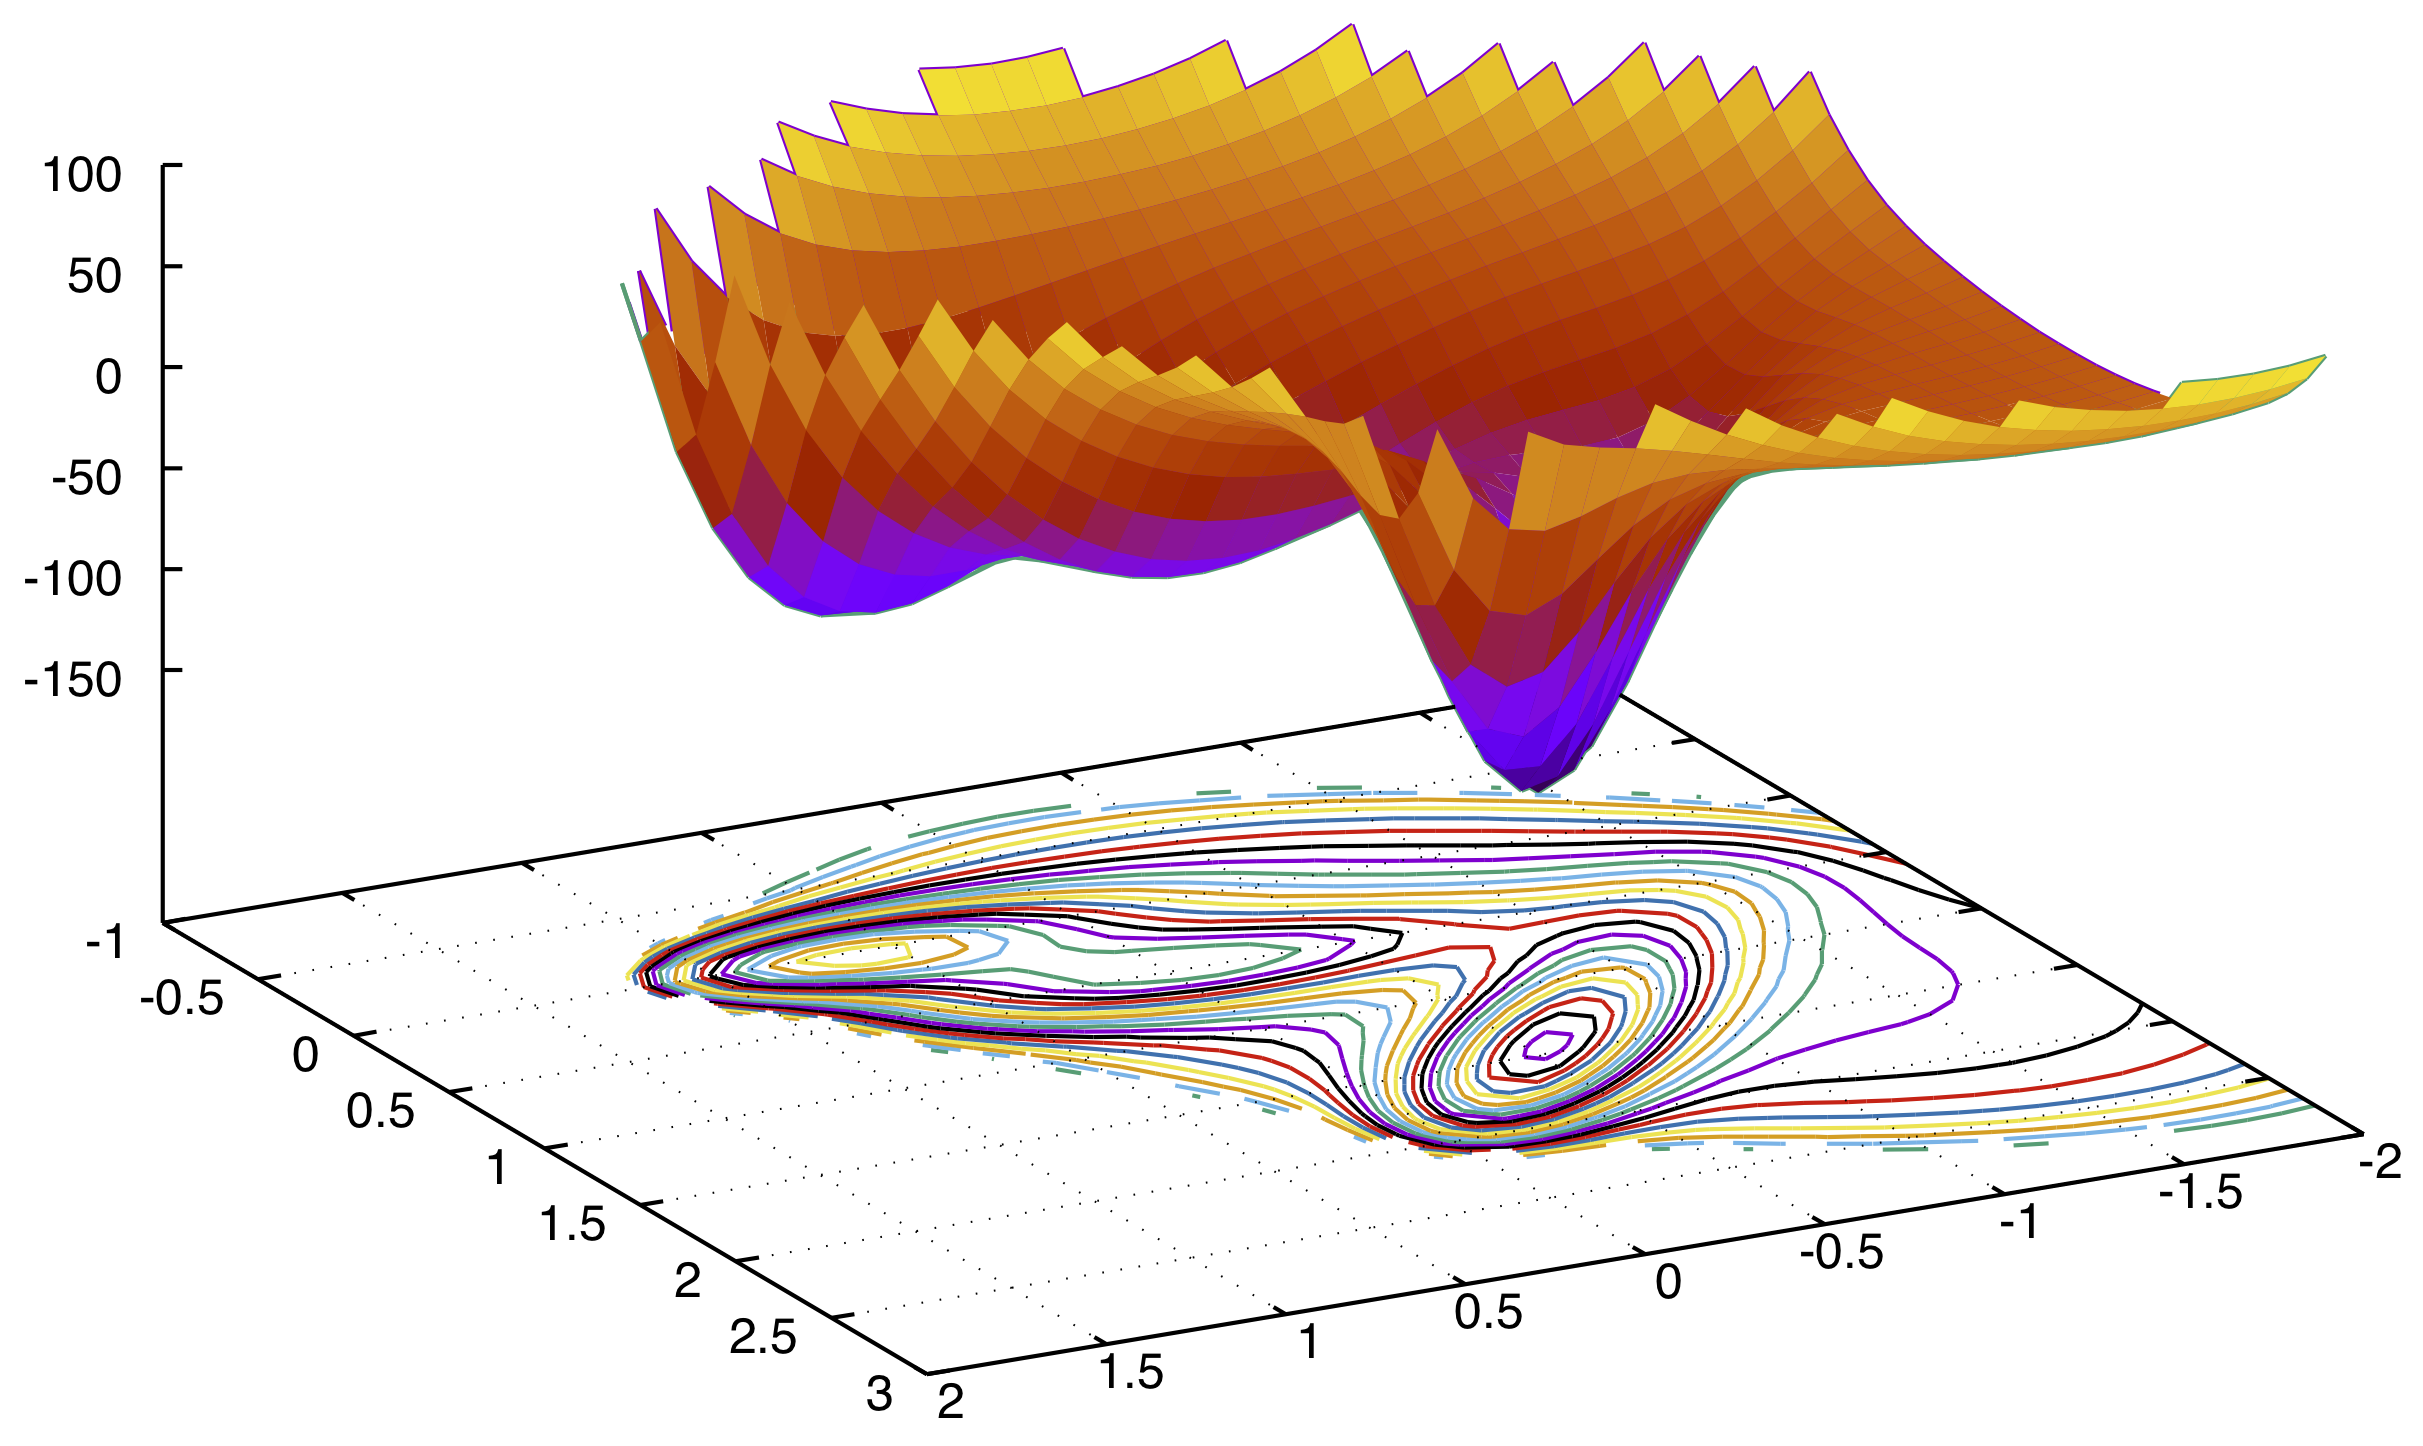
\includegraphics[width=.5\textwidth]{12.png}
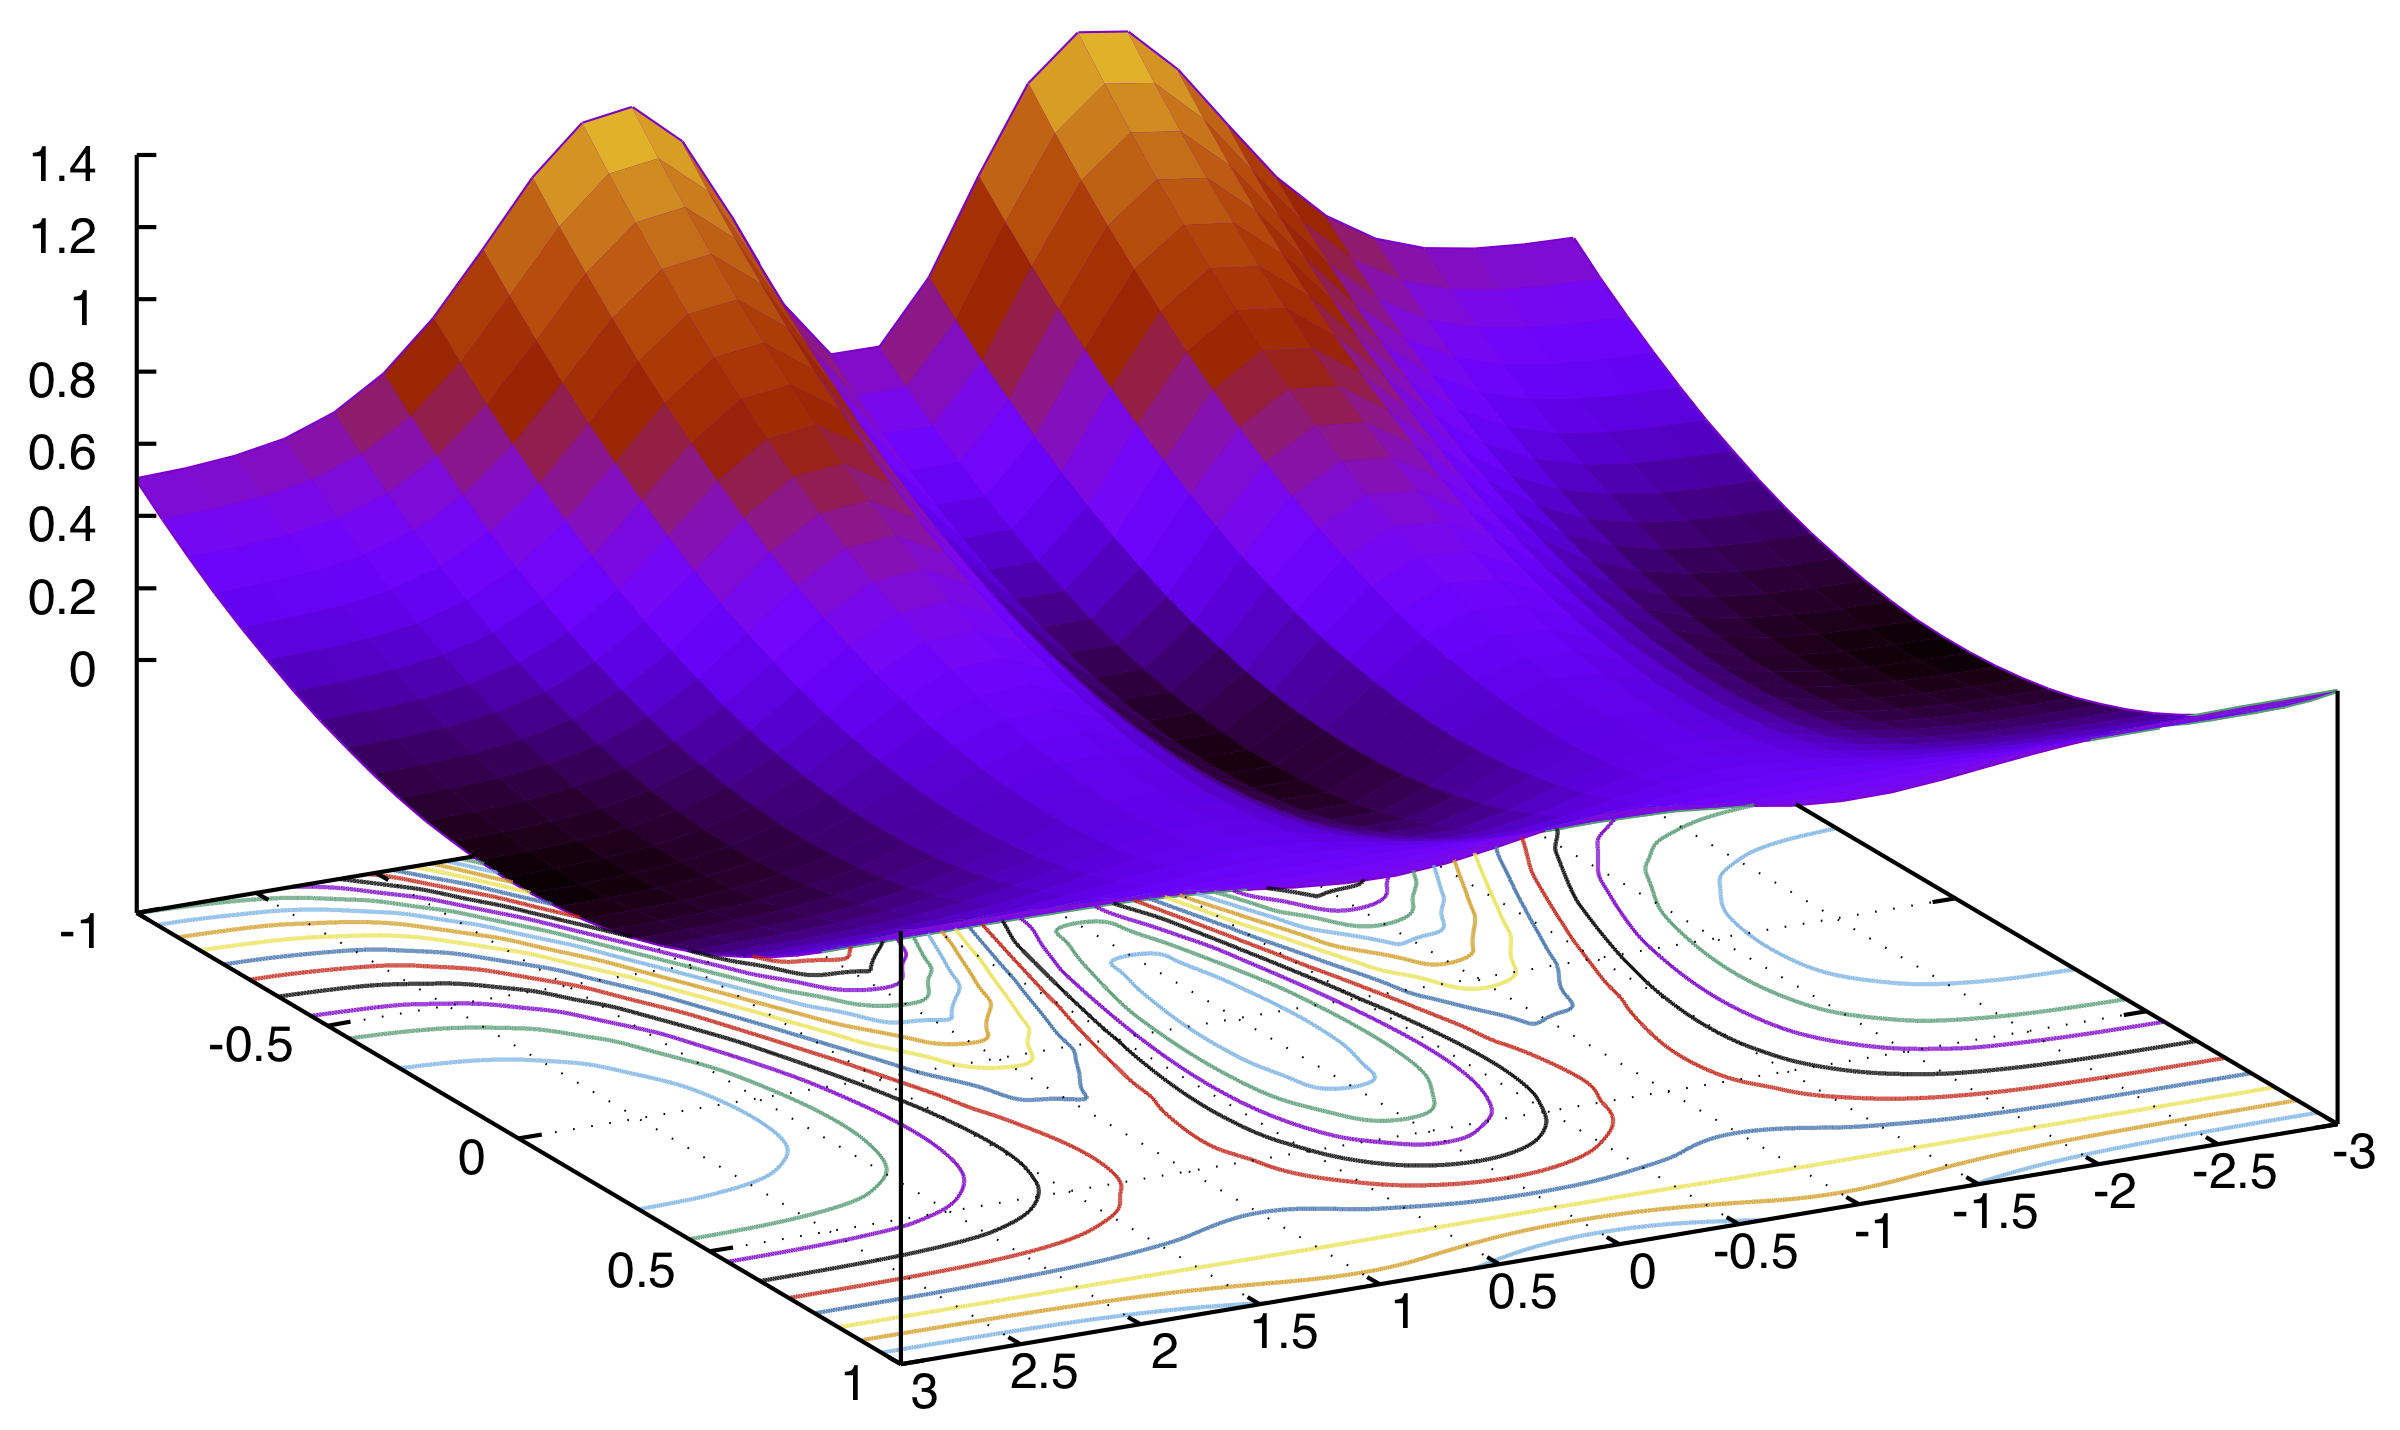
\includegraphics[width=.5\textwidth]{13.png}
%\footnotesize
%\begin{pyglist}[language=python,fvset={frame=single}]
%\end{pyglist}

\input{mpi}
\normalsize
\subsection[\_shm]{\_shm.so}
This binary module (must be compiled) provides basic SHM functionality within python.\\
The shared memory can be reserved via python script (\func{alloc}) or directly accessed once known the allocation identifier (\parm{shmid}).
The main purpose of this module is to speed-up the communication layer with third party programs (engines), removing the need for
physical files (SHM works directly on RAM) to communicate with the external engines (ie, updating partial charges, coordinates, gradients, ...).\\
It provides 2 basic mechanisms: \parm{read}/\parm{write} in which binary strings (bytes) are managed (and parsed/generated using the struct.pack/unpack mechanism), or direct acces to lists of floats (\parm{read\_r8}/\parm{write\_r8}).
\begin{pyglist}[language=python,fvset={frame=single}]
shmid = _shm.alloc( size_in_bytes )

_shm.clean( shmid )

_shm.write( shmid, "bytes" )

"" = _shm.read( shmid, size_in_bytes )

_shm.write_r8( shmid, [ float ] )

[ float ] = _shm.read_r8( shmid, num_of_floats )
\end{pyglist}

\footnotesize
\begin{pyglist}[language=python,fvset={frame=single}]
import qm3.utils._shm
import struct

n = 10
p = qm3.utils._shm.alloc( n * 8 )

qm3.utils._shm.write( p, b"".join( [ struct.pack( "d", i ) for i in range( n ) ] ) )
print( qm3.utils._shm.read_r8( p, n ) )

qm3.utils._shm.write_r8( p, [ float( i ) for i in range( n ) ] )
print( list( struct.unpack( "%dd"%( n ), qm3.utils._shm.read( p, n * 8 ) ) ) )

qm3.utils._shm.clean( p )
\end{pyglist}

%\begin{pyglist}[fvset={frame=single}]
%#SOURCE@../samples/logs/
%\end{pyglist}

\input{free_energy}
\input{prepare}

\section{qm3.io}
\normalsize
\subsection[dcd]{dcd.py}
The class \func{dcd} provides
minimal methods for reading and writing XPLOR-based trajectory files (DCD). The main variables/attributes are
the number of atoms (\func{N}); and the coordinates (\func{X}, \func{Y} and \func{Z}), which should
be modified previous to an \func{append} call. The \func{read} and \func{write} methods are intended
only for initialisation, and \func{next}/\func{append} will perform the reading/writing sutff.
The final number of frames in the trajectory is set after the \func{close} method is called.\\
\begin{pyglist}[language=python,fvset={frame=single}]
class dcd( fname = None, qprint = True )
    N = 0
    X = []
    Y = []
    Z = []
    def read( fname, qprint = True )
    def next()
    def close()
    def write( fname, natoms, sele = None )
    def append()
\end{pyglist}

\normalsize
\subsection[mol2]{mol2.py}
Basic parser for MOL2 file types. It returns both the molecule and the list of bonds of the molecule.
\begin{pyglist}[language=python,fvset={frame=single}]
def mol2_read( fname = None )
\end{pyglist}

\normalsize
\subsection[sdf]{sdf.py}
Internet database accessing (\func{db\_download}: where \parm{code} is a pair composed by the server and the molecule
identifier, such as "pubchem:12039" / ":12039" or "chemspider:4573889").
\begin{pyglist}[language=python,fvset={frame=single}]
def sdf_read( fname = None )
def db_download( code )
\end{pyglist}


\section{qm3.actions}
\input{minimize}
\input{genetic}
\input{paths}
\input{dynamics}
\input{fitting}
\input{string}
\normalsize
\subsection[grote\_hynes]{grote\_hynes.py}

\begin{pyglist}[language=python,fvset={frame=single}]
class grote_hynes( obj, coordinate, step_size = 0.0005, print_frequency = 100,
         project_RT = True, step_number = -1, log_function = default_log )
	def integrate()
	def stats()

class coordinate_antisymmetric( atoms )
	def stop()
	def value( coor )
	def force( mass, coor, grad )
	def constraint( mass, coor, fvel, velo, facc, acce, flmb, refc )

class coordinate_bond( atoms )
	def stop()
	def value( coor )
	def force( mass, coor, grad )
	def constraint( mass, coor, fvel, velo, facc, acce, flmb, refc )
\end{pyglist}

\footnotesize
\begin{pyglist}[language=python,fvset={frame=single}]
\end{pyglist}

\input{vina}
\input{ipi}

\section{qm3.engines}
The following strings: \textbf{qm\_job} (energy, gradient, ...), \textbf{qm3\_guess} (whether
a previous wavefunction can be read), \textbf{qm3\_atoms} (symbols and coordinates for the QM atoms) and
\textbf{qm3\_charges} (coordinates and charges of the MM atoms), are common replacements
in QM input templates. In addition, other strings can also be defined depending on a particular program,
such as \textbf{qm3\_nchg} (DFTB+: total amount of MM charges within the QM calculation)
or \textbf{qm3\_field} (Gaussian: points where calcualting the electric field generated by
the QM atoms and the wave-function).\\
The base module offers the function \func{exclussions}, which helps in defining those 
MM terms that should be added whenever a QM-MM partition (using the Link Atom approach) is performed.
\begin{pyglist}[language=python,fvset={frame=single}]
def exclussions( sele_QM, molec, bonds = None )
\end{pyglist}
\input{mmres}
\input{colvar_v}
\input{colvar_s}
\input{plumed}
\input{mmint}
% -- MM
\input{mol_mech}
\input{charmm}
\input{dynamo}
\input{namd}
\input{sander}
\input{lammps}
\input{openmm}
\input{gromacs}
% -- QM_semi
\input{dftb}
\input{sqm}
% -- QM_abin
\input{demon}
\input{gamess}
\input{gaussian}
\input{lsdalton}
\input{nwchem}
\input{orca}
\input{psi4}
\input{qchem}
\input{smash}
\input{tmole}
\input{tchem}
\input{bagel}

\section{Testcase: Oxy-cope in water}
\input{oxy_pes}
\input{oxy_ts}
\input{oxy_pmf}
\end{document}
